\section{Experiment Design} %#TODO: Refactoring
%#TODO: Think if adding Self-solve agent and KB Gaps Analysis
\subsection{Introduction}
Any measurement, without knowledge of the uncertainty, is \textbf{meaningless}.
Here, "meaningless" means a measurement lacks reliability if its uncertainty is unknown; without knowing its precision or accuracy, the value cannot be trusted or interpreted and may be \textbf{misleading}.

Experimental measurements are essential to understand system behavior, allowing us to:
\begin{itemize}
    \item Decide to \textbf{ship or not}
    \item \textbf{Identify} improvements for next iterations
    \item \textbf{Communicate} system behavior to others
\end{itemize}
This enables estimation of system performance for properties and conditions of interest.

We focus on experimenting rather than just evaluating or testing because:
\begin{itemize}
    \item We always use a data sample, lacking access to all or future data
    \item Results vary due to factors beyond the dataset (workflow, randomness, etc.)
\end{itemize}

We can experiment with various LLM system components:
\begin{itemize}
    \item \textbf{Document Base}: quality of the knowledge base or corpus
    \item \textbf{Retrieval Algorithm}: effectiveness in finding information
    \item \textbf{LLM Answer Generation}: quality of answers from context
\end{itemize}
Isolating what to test is harder than in traditional software due to interdependent components and less control.
Some measures are end-to-end (whole system), others pinpoint where to intervene.

If done and reported correctly, more experiments provide more information; otherwise, they introduce bias.

Before starting, define uncertainty using basic probability principles.

\subsection{Basic, Probabilities and Random Variables}

\subsubsection{Definition of Probability}
From a general perspective, probability is a number between 0 and 1 to which we assign a meaning.
A frequentist defines it as "\textit{A proportion (\# of times an event occurs)/repetitions as experiments repetitions tends to infinity}".
However, this approach cannot work with us, since we cannot repeat experiments infinitely, and we cannot experiment always in the same conditions.

So, more generally the definition on which we are interested is "\textit{A belief/likelihood of an event occurring}" or  "\textit{a belief on the distribution of a random variable}".

More formally we define:
\begin{itemize}
    \item \textbf{Sample Space (S)}: The set of all possible outcomes of an experiment.
    \item \textbf{Outcome}: An outcome is a single element of the sample space.
    \item \textbf{Event (E)}: An event is a subset of the sample space that satisfies some conditions.
\end{itemize}

We define $P(E)$ as the probability of an event $E$ occurring, and we have the following axioms:

More formally, we can define the two interpretations of probability as follows:
\begin{itemize}
    \item \textbf{Frequentist Interpretation}: \[ P(E) = \lim_{n \to \infty} n(E)/n \]
    where $n(E)$ is the number of times event $E$ occurs in $n$ trials.
    \item \textbf{Bayesian Interpretation}: \[ P(E) = P(E | I) = belief\]
    where $I$ is the background information and belief is a subjective degree of confidence in the occurrence of event $E$.
    This can be seen as an estimation of the frequentist probability, where the belief is updated as new evidence is obtained, following Bayes' theorem.
\end{itemize}

\subsubsection{Axioms of Probability}
For both interpretations, we have the following axioms of probability:
\begin{itemize}
    \item \textbf{Non-negativity}: $P(E) \geq 0 \forall E \in S$.
    \item \textbf{Normalization}: $P(S) = 1$.
    \item \textbf{Complement Rule}: $P(E') = 1 - P(E)$, where $E'$ is the complement of $E$.
\end{itemize}

Then if an event $E$ is \textbf{mutually exclusive} with another event $F$ (i.e., they cannot occur simultaneously), we have:
\begin{equation}
    P(E \cup F) = P(E) + P(F)
\end{equation}
This is the simplest case, and can be extended to more than two events.

In the case we have all outcomes \textbf{equally likely}, we can calculate the probability of an event $E$ as:
\begin{equation}
    P(E) = \frac{|E|}{|S|}
\end{equation}
And works only if we have a finite sample space, and all outcomes are equally likely.

\subsubsection{Random Variables}
We define a \textbf{random variable} as a function that maps each outcome of an experiment to a real number, capturing uncertainty.
Assigning a value to a random variable defines an event, and we can describe its behavior with a probability distribution.

For example, in a coin toss, let $X$ be 1 for heads and 0 for tails.
This is a \textbf{binary random variable} since it takes two values.
If both outcomes are equally likely, the probability distribution is:
\begin{equation}
    P(X=1) = 0.5, \quad P(X=0) = 0.5
\end{equation}

\paragraph{Probability Mass Function (PMF)}
The \textbf{probability mass function (PMF)} of a discrete random variable gives the probability that it equals a specific value: $P(X=k)$ for each possible $k$.
The PMF represents the distribution and allows calculation of event probabilities.

\subsection{Foundational Random Variables}
Some random variables are classic and foundational in probability theory.
They can be used to model various phenomena and are essential for understanding uncertainty in experiments.

\subsubsection{Binomial Random Variable}
The scenario we are describing is the following: 
\begin{itemize}
    \item $n$ independent trials
    \item A consistent probability of success $p$ in each trial, binary outcomes (success/failure)
    \item We want the probability of observing $k$ successes in those $n$ trials
\end{itemize}
The probability of observing $k$ successes in $n$ trials is given by the \textbf{binomial distribution}:
\begin{equation}
    X \sim Bin(n, p)
\end{equation}
Where $X$ is the random variable representing the number of successes, and its PMF is:
\begin{equation}
    P(X=k) = \binom{n}{k} p^k (1-p)^{n-k}
\end{equation}
Where $\binom{n}{k}$ is the binomial coefficient, calculated as:
\begin{equation}
    \binom{n}{k} = \frac{n!}{k!(n-k)!}
\end{equation}
The binomial distribution is useful for modeling scenarios like coin tosses.

If we plot the PMF of a binomial distribution with $n=10$ and $p=0.5$, we would see a bell-shaped curve centered around $k=5$, indicating that observing 5 successes is the most likely outcome.

\begin{figure}[h]
    \centering
    % Binomial PMF plot for n=10, p=0.5
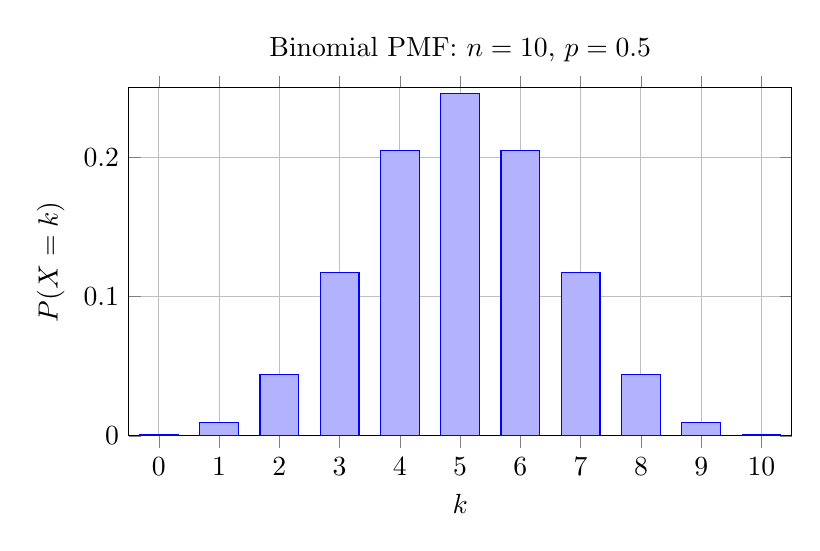
\begin{tikzpicture}
    \begin{axis}[
        ybar,
        bar width=14pt,
        ymin=0,
        ymax=0.25,
        xmin=-0.5,
        xmax=10.5,
        xtick={0,1,2,3,4,5,6,7,8,9,10},
        xlabel={$k$},
        ylabel={$P(X=k)$},
        title={Binomial PMF: $n=10$, $p=0.5$},
        width=10cm,
        height=6cm,
        grid=major
    ]
    \addplot+[blue,fill=blue!30] coordinates {
        (0,0.00098)
        (1,0.00977)
        (2,0.04395)
        (3,0.11719)
        (4,0.20508)
        (5,0.24609)
        (6,0.20508)
        (7,0.11719)
        (8,0.04395)
        (9,0.00977)
        (10,0.00098)
    };
    \end{axis}
\end{tikzpicture}
    \caption{PMF of the binomial distribution with $n=10$, $p=0.5$}
\end{figure}

\subsubsection{Bernoulli Random Variable}
The Bernoulli distribution is a special case of the binomial distribution where $n=1$.
It models a single trial with two possible outcomes: success (1) with probability $p$ and failure (0) with probability $1-p$.
The PMF of a Bernoulli random variable $X$ is:
\begin{equation}
    P(X=1) = p, \quad P(X=0) = 1-p
\end{equation}

\subsubsection{Other PMFs Random Variables}
Other important discrete random variables include:
\begin{itemize}
    \item \textbf{Geometric}: Models the number of trials until the first success in a sequence of independent Bernoulli trials.
    \[ P(X=k) = (1-p)^{k-1} p \]
    \item \textbf{Negative Binomial}: Models the number of trials until a specified number of successes occurs.
    \[ P(X=k) = \binom{k-1}{r-1} p^r (1-p)^{k-r} \]
\end{itemize}